% Artigo escrito em junho de 2007
% Por Caroline Vicentini e Ronaldo Canofre
% Revisao da Professora Tutora Andrea Charao
\documentclass[12pt]{article}

\usepackage{ref/sbc-template}
\usepackage{graphicx,url}
\usepackage[brazil]{babel}   
\usepackage[latin1]{inputenc}  
\usepackage{xspace}
     
\sloppy

\title{Desenvolvimento de uma Biblioteca Digital\\ de Trabalhos de Gradua\c{c}\~{a}o}

\author{Adler Hoff Schmidt\inst{1}, Caroline Figueira Vicentini\inst{1}, Fernando Bevilacqua\inst{1}, \\Ronaldo Canofre M. dos Santos \inst{1}, Andrea Schwertner Char\~{a}o\inst{1} }


\address{Programa de Educa\c{c}\~{a}o Tutorial (PET) -- Curso de Ci\^{e}ncia da Computa\c{c}\~{a}o\\
  Universidade Federal de Santa Maria (UFSM)
  \email{\{adlerhs, carol, fernando, canofre, andrea\}@inf.ufsm.br}
}

\newcommand{\software}{\textit{software}\xspace}
\newcommand{\site}{\textit{site}\xspace}

\begin{document}

\maketitle

     
\begin{resumo}
O acesso aos resultados das pesquisas e trabalhos realizados nas universidades \'{e} importante para que o conhecimento seja disseminado e a ci\^{e}ncia, a tecnologia e a sociedade continuem evoluindo. Neste artigo, tem-se como foco a divulga\c{c}\~{a}o de trabalhos elaborados pelos acad\^{e}micos do Curso de Ci\^{e}ncia da Computa\c{c}\~{a}o da Universidade Federal de Santa Maria (UFSM). Com o objetivo de disseminar e compartilhar informa\c{c}\~{o}es sobre estes trabalhos, desenvolveu-se um sistema que permite gerenciar uma biblioteca digital de trabalhos de gradua\c{c}\~{a}o atrav\'{e}s da Web. Para implementa\c{c}\~{a}o desse sistema, utilizou-se as tecnologias MySQL e PHP5, que s\~{a}o amplamente difundidas atualmente. O resultado obtido foi um sistema de divulga\c{c}\~{a}o de trabalhos de gradua\c{c}\~{a}o que pode ser facilmente adaptado para problemas semelhantes e utilizado por outros cursos e outras universidades~\nocite{sbc}.
\end{resumo}


\section{Introdu\c{c}\~{a}o}
Os resultados de trabalhos realizados em universidades precisam ser compartilhados com a sociedade e com o meio acad\^{e}mico do qual fazem parte. Isso permite disseminar o conhecimento adquirido ao desenvolver-se tais trabalhos, proporcionando assim o crescimento das \'{a}reas envolvidas. Tradicionalmente, esse compartilhamento \'{e} proporcionado pelas bibliotecas universit\'{a}rias, que mant\^{e}m em seus acervos as monografias, disserta\c{c}\~{o}es e teses produzidas nas institui\c{c}\~{o}es. Com o avan\c{c}o tecnol\'{o}gico, surgiu tamb\'{e}m a possibilidade de armazenar e disponibilizar informa\c{c}\~{o}es sobre esses trabalhos digitalmente, facilitando assim o acesso ao p\'{u}blico.

Atualmente, existem esfor\c{c}os do governo em reunir e divulgar as disserta\c{c}\~{o}es e teses desenvolvidas nos cursos de p\'{o}s-gradua\c{c}\~{a}o do pa\'{i}s. Um exemplo desses esfor\c{c}os \'{e} a Biblioteca Digital de Teses e Disserta\c{c}\~{o}es (BDTD)~\cite{bdtd}, que \'{e} um projeto que busca integrar os sistemas de informa\c{c}\~{a}o das universidades brasileiras e incentivar a divulga\c{c}\~{a}o das teses e disserta\c{c}\~{o}es em meio digital. Seguindo esta tend\^{e}ncia, os cursos de gradua\c{c}\~{a}o v\^{e}m tamb\'{e}m se preocupando em melhorar a dissemina\c{c}\~{a}o de seus trabalhos tanto interna como externamente ao meio universit\'{a}rio~\cite{avaliacao}.

Os alunos do Curso de Ci\^{e}ncia da Computa\c{c}\~{a}o da UFSM produzem Trabalhos de Gradua\c{c}\~{a}o (TG's) como requisito para integraliza\c{c}\~{a}o curricular. Os assuntos abordados nesses trabalhos s\~{a}o de interesse da comunidade acad\^{e}mica e geralmente apresentam resultados de pesquisas desenvolvidas na \'{a}rea de computa\c{c}\~{a}o, dentro da institui\c{c}\~{a}o. Embora esses trabalhos possam ser consultados nas bibliotecas da universidade, entende-se que o acesso aos mesmos poderia ser facilitado atrav\'{e}s de sistemas de informa\c{c}\~{a}o especialmente concebidos para este fim.

Observando este cen\'{a}rio que \'{e} tamb\'{e}m recorrente em outros cursos e universidades, o grupo PET-CC (Programa de Educa\c{c}\~{a}o Tutorial do Curso de Ci\^{e}ncia da Computa\c{c}\~{a}o)~\cite{sesu} juntamente com a coordena\c{c}\~{a}o do curso, buscou uma solu\c{c}\~{a}o para melhorar a dissemina\c{c}\~{a}o dos TG's produzidos. Ap\'{o}s uma an\'{a}lise do problema e das solu\c{c}\~{o}es existentes, decidiu-se desenvolver um sistema para gerenciamento de uma biblioteca digital de TG's atrav\'{e}s da Web.

Este artigo apresenta o processo de desenvolvimento do referido sistema. Para isso, descreve-se primeiramente a etapa de an\'{a}lise do problema e as medidas adotadas para o levantamento de requisitos do sistema. Em seguida, discute-se o projeto do sistema, detalhando-se a modelagem de seus elementos. Na seq\"{u}\^{e}ncia, apresenta-se a etapa de implementa\c{c}\~{a}o do sistema, descrevendo-se as ferramentas utilizadas e os testes realizados para verifica\c{c}\~{a}o do funcionamento do sistema. Para finalizar, apresenta-se uma avalia\c{c}\~{a}o dos resultados obtidos at\'{e} o momento, seguida da conclus\~{a}o do trabalho.


\section{An\'{a}lise do Problema e Levantamento de Requisitos}

O ponto de partida para o trabalho foi a defini\c{c}\~{a}o dos objetivos do sistema: divulgar os TG's de maneira eficiente ao p\'{u}blico interessado e prover meios para manter atualizadas as informa\c{c}\~{o}es no sistema.

Para atingir o primeiro objetivo, decidiu-se divulgar os trabalhos ao p\'{u}blico atrav\'{e}s da Web, pois esta tecnologia se tornou amplamente popular e permite acesso \`{a} dist\^{a}ncia sem necessidade de instala\c{c}\~{a}o de \software por parte dos usu\'{a}rios. Al\'{e}m disso, esta op\c{c}\~{a}o permite a integra\c{c}\~{a}o do sistema com o \site Web do Curso de Ci\^{e}ncia da Computa\c{c}\~{a}o, o que facilita a divulga\c{c}\~{a}o dos TG's \`{a}s pessoas interessadas na \'{a}rea de computa\c{c}\~{a}o na UFSM. Decidiu-se tamb\'{e}m permitir a divulga\c{c}\~{a}o do conte\'{u}do integral dos trabalhos, e n\~{a}o apenas resumos dos mesmos.

Para suprir a necessidade de manter o sistema atualizado, decidiu-se incluir a funcionalidade de administra\c{c}\~{a}o do sistema atrav\'{e}s da Web. Deste modo, \'{e} poss\'{i}vel atualizar o conte\'{u}do do sistema em qualquer local e de forma independente do sistema operacional utilizado.

Durante a etapa de defini\c{c}\~{o}es do sistema, realizou-se reuni\~{o}es com o coordenador do curso para melhor compreender o problema. Nesta etapa, analisou-se o processo de tramita\c{c}\~{a}o dos TG's no Curso e definiu-se os dados relevantes a serem divulgados, as pessoas que teriam permiss\~{a}o para atualizar o sistema, entre outras informa\c{c}\~{o}es.

A partir da especifica\c{c}\~{a}o dos objetivos e funcionalidades do sistema, realizou-se um levantamento de ferramentas existentes que poderiam se utilizadas e/ou adaptadas para suprir as necessidades identificadas. Dentre os sistemas encontrados, destacam-se o Sistema de Publica\c{c}\~{a}o Eletr\^{o}nica de Teses e Disserta\c{c}\~{o}es - TEDE~\cite{tede} e o Sistema NOU-RAU~\cite{nourau}.

Embora esses sistemas contemplem a maioria das funcionalidades desejadas e at\'{e} mesmo as superem, notou-se que a utiliza\c{c}\~{a}o desses sistemas poderia trazer algumas dificuldades. Em primeiro lugar, seria trabalhoso integrar esses sistemas com o \site do Curso, mantendo-se a identidade visual e a similaridade das interfaces com os usu\'{a}rios. Al\'{e}m disso, o uso de sistemas existentes poderia reduzir a liberdade da coordena\c{c}\~{a}o do Curso no gerenciamento dos TG's. Por fim, a adapta\c{c}\~{a}o desses sistemas \`{a}s necessidades espec\'{i}ficas ao gerenciamento de TG's poderia exigir um esfor\c{c}o consider\'{a}vel de compreens\~{a}o e modifica\c{c}\~{a}o de c\'{o}digo.

Tendo em vista os fatores acima mencionados, decidiu-se desenvolver um sistema sob medida para a biblioteca digital de TG's. No entanto, teve-se o cuidado de projetar um sistema flex\'{i}vel que possa ser adaptado a novos requisitos que surjam durante ou ap\'{o}s o desenvolvimento, e que possa ser reutilizado por outros cursos e universidades. O sistema foi chamado de Biblioteca Digital de Trabalhos de Gradua\c{c}\~{a}o (BDTG).


\section{Projeto}
Ap\'{o}s o levantamento dos dados necess\'{a}rios para o desenvolvimento do sistema, iniciou-se o projeto atrav\'{e}s da modelagem da base de dados com as informa\c{c}\~{o}es referentes aos TG's. O diagrama UML \'{e} mostrado na figura \ref{f:diagrama-uml}.

\begin{figure}[ht]
\centering
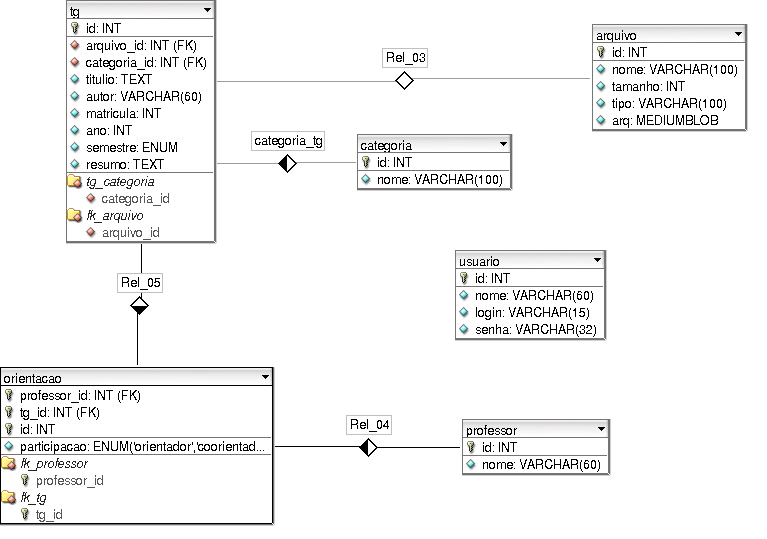
\includegraphics [width = 0.9\textwidth]
{img/diagrama.png}
\caption{Diagrama UML da Base de Dados da BDTG}
\label{f:diagrama-uml}
\end{figure}

A principal tabela do sistema \'{e} denominada \texttt{tg}. Esta tabela armazena as informa\c{c}\~{o}es relevantes sobre os trabalhos desenvolvidos, como por exemplo o nome do autor, o t\'{i}tulo e o resumo do trabalho. Devido ao fato de um professor poder ser orientador de v\'{a}rios trabalhos, decidiu-se criar uma tabela separada somente para os professores. Uma caracter\'{i}stica espec\'{i}fica do sistema \'{e} que um trabalho pode ter um orientador e um co-orientador, sendo por esse motivo adotado um sistema N-N entre as tabelas \texttt{professor} e \texttt{tg}. Na tabela resultante deste relacionamento, fica armazenada a informa\c{c}\~{a}o sobre o tipo de participa\c{c}\~{a}o do professor no trabalho em quest\~{a}o. Caso n\~{a}o existisse a co-orienta\c{c}\~{a}o nos trabalhos de gradua\c{c}\~{a}o, o professor poderia se relacionar com a tabela \texttt{tg} atrav\'{e}s de uma chave estrangeira.

A tabela \texttt{arquivo} armazena o texto integral de cada TG, geralmente em formato PDF. Esta tabela tem um relacionamento 1-1 com a tabela \texttt{tg}, podendo ser englobado por esta. No entanto, optou-se por utilizar uma tabela separada no sistema por tr\^{e}s motivos principais: (a) devido ao arquivo ter caracter\'{i}sticas de uma entidade independente; (b) por ele armazenar o bin\'{a}rio do TG, que geralmente \'{e} um campo muito grande para ser inclu\'{i}do em consultas; e (c) porque alguns TG's poderiam n\~{a}o ter o arquivo em vers\~{a}o PDF dispon\'{i}vel, seja por motivos de sigilo ou por perda de arquivos. A tabela \texttt{categorias} foi criada para dar ao usu\'{a}rio a possibilidade de pesquisar TG's com algum assunto em comum. Um TG pode somente ser associado a uma categoria e uma categoria pode estar associada a v\'{a}rios TG's. As informa\c{c}\~{o}es sobre alunos n\~{a}o foram armazenadas em uma tabela separada porque os alunos n\~{a}o publicam mais de um TG em um mesmo curso e tamb\'{e}m por que os TG's devem ser desenvolvidos individualmente. Sendo assim, decidiu-se incluir o nome e a matr\'{i}cula do aluno como campos da tabela \texttt{tg}.

A tabela \texttt{usuario} foi criada para que uma ou mais pessoas pudessem ter acesso ao sistema e tamb\'{e}m para garantir o acesso restrito ao sistema pelas pessoas que tem permiss\~{a}o para isso. Esta tabela n\~{a}o se relaciona com nenhuma outra tabela.

Ap\'{o}s a modelagem de dados, escolheu-se o sistema gerenciador da base de dados para armazenar as informa\c{c}\~{o}es do sistema. Nesse caso, optou-se por utilizar o MySQL~\cite{mysql} por ser um gerenciador amplamente difundido e documentado. Al\'{e}m disso, servidores MySQL j\'{a} encontravam-se instalados no servidor Web do NCC (N\'{u}cleo de Ci\^{e}ncia da Computa\c{c}\~{a}o), que hospeda atualmente o \site do Curso de Ci\^{e}ncia da Computa\c{c}\~{a}o, e no servidor do grupo PET - Ci\^{e}ncia da Computa\c{c}\~{a}o (PET-CC), que hospedaria o sistema durante a fase de implementa\c{c}\~{a}o. 

Seguindo com o planejamento do sistema, decidiu-se utilizar o paradigma de orienta\c{c}\~{a}o a objetos para o desenvolvimento. Essa escolha deveu-se ao fato de que sistemas desenvolvidos utilizando classes s\~{a}o mais f\'{a}ceis de codificar e, principalmente, de alterar futuramente. A linguagem PHP5~\cite{php} foi escolhida principalmente por suportar orienta\c{c}\~{a}o a objetos e tamb\'{e}m por existir um servidor Apache com suporte a PHP tanto no NCC quando no grupo PET-CC. Al\'{e}m disso, a equipe de desenvolvimento j\'{a} possuía conhecimento e experi\^{e}ncia no desenvolvimento de sistemas utilizando essa linguagem.


\section{Implementa\c{c}\~{a}o}

Para fins de organiza\c{c}\~{a}o do c\'{o}digo do sistema, decidiu-se separ\'{a}-lo em duas partes: uma para disponibilizar os TG's ao p\'{u}blico e outra para gerenciar as informa\c{c}\~{o}es do sistema. Os arquivos de ambos sistemas utilizam as mesmas classes para manipular os objetos e a base de dados, apenas os arquivos que processam os dados e os que mostram os dados na tela ficam em pastas separadas. Isso permite mover os arquivos de lugar, mantendo o sistema funcionando apenas alterando os arquivos de configura\c{c}\~{a}o.

Tamb\'{e}m decidiu-se organizar o c\'{o}digo separando-o em arquivos diferentes segundo sua fun\c{c}\~{a}o l\'{o}gica e tamb\'{e}m separar os arquivos que possuem a mesma funcionalidade para o sistema. Assim, o sistema ficou dividido em diret\'{o}rios, como mostra a figura \ref{f:arvore-dir}.

\begin{figure}[ht]
\centering
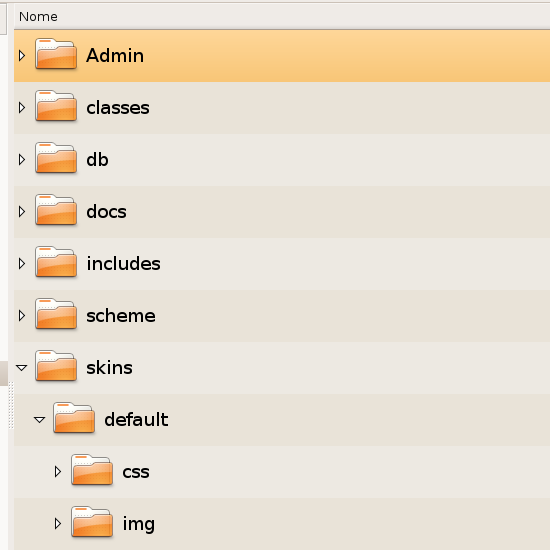
\includegraphics [width = 6cm, height = 6cm]
{img/arvoreDir.png}
\caption{\'{A}rvore de Diret\'{o}rios do Sistema}
\label{f:arvore-dir}
\end{figure}

No diret\'{o}rio \texttt{classes} ficam os arquivos que manipulam os objetos; no diret\'{o}rio \texttt{skins} ficam as pastas contendo os layouts do sistema\footnote{Atualmente, h\'{a} apenas um layout desenvolvido, que fica na pasta \texttt{default}}; na pasta \texttt{db} ficam os arquivos que manipulam a base de dados; no diret\'{o}rio \texttt{docs} fica a documenta\c{c}\~{a}o do sistema; no diret\'{o}rio \texttt{includes} fica um arquivo respons\'{a}vel por fazer a inclus\~{a}o dos arquivos necess\'{a}rio em todos os arquivos do sistema; no diret\'{o}rio \texttt{scheme} fica um arquivo com o c\'{o}digo SQL de cria\c{c}\~{a}o da base de dados; o diret\'{o}rio \texttt{testes} armazena arquivos de exemplo e arquivos para testes do sistema; no diret\'{o}rio raiz ficam os arquivos que processam as informa\c{c}\~{o}es fornecidas pelos usu\'{a}rios.

A implementa\c{c}\~{a}o foi realizada por uma equipe de tr\^{e}s programadores. Para organizar o trabalho, definiu-se regras referentes \`{a} codifica\c{c}\~{a}o, \`{a} armazenagem do sistema, divis\~{a}o e controle de tarefas, reuni\~{o}es e testes.

Para implementar o sistema, optou-se por dividir as classes e arquivos entre os integrantes da equipe de desenvolvimento. As classes foram implementadas separadamente, mas os programas foram testados todos juntos durante reuni\~{o}es de testes. Sabia-se de antem\~{a}o que esta abordagem poderia acarretar problemas como c\'{o}digo inconsistente e perda de informa\c{c}\~{o}es. Assim, decidiu-se utilizar um sistema de controlador de vers\~{o}es, o SVN~\cite{svn}, que possibilitou que cada integrante desenvolvesse seus c\'{o}digos em diferentes computadores, mas tendo sempre a vers\~{a}o atual das classes e arquivos corrigidos. O SVN foi instalado no servidor do PET-CC.

A cada divis\~{a}o de tarefas de implementa\c{c}\~{a}o, definiu-se um prazo para conclus\~{a}o dessas tarefas. Para facilitar o gerenciamento do processo de desenvolvimento, utilizou-se o sistema gerenciador de tarefas NetOffice~\cite{netoffice}, que j\'{a} estava sendo utilizado pelo grupo PET-CC para gerenciar suas atividades internas e atividades de grupo.

Cada tabela da base de dados deu origem a uma classe. No m\'{o}dulo de administra\c{c}\~{a}o, as funcionalidades implementadas foram: inclus\~{a}o/altera\c{c}\~{a}o/exclus\~{a}o/busca de TG's, professores, arquivos e usu\'{a}rios; possibilidade de relacionar TG's com professores atrav\'{e}s da tabela orienta\c{c}\~{a}o e possibilidade de visualizar os dados cadastrados no sistema. No m\'{o}dulo acessível aos demais usu\'{a}rios, as funcionalidades resumem-se \`{a} pesquisa de TG's, que pode ser realizada de 3 formas: atrav\'{e}s de palavras-chave preenchidas em um formul\'{a}rio de busca, atrav\'{e}s de uma op\c{c}\~{a}o que busca os \'{u}ltimos tgs produzidos ou atrav\'{e}s das categorias de TG's presentes na base de dados. O usu\'{a}rio tem tamb\'{e}m a possibilidade de visualizar o arquivo do TG caso este esteja dispon\'{i}vel.

O layout inicial do sistema \'{e} baseado no layout do \site do curso de Ci\^{e}ncia da Computa\c{c}\~{a}o, para garantir maior integra\c{c}\~{a}o entre os sistemas. \'{E} poss\'{i}vel  alterar o layout apenas incluindo uma nova pasta no diret\'{o}rio \texttt{skins} e alterando o arquivo de configura\c{c}\~{a}o.

Durante a implementa\c{c}\~{a}o do sistema, realizou-se diversos testes e corre\c{c}\~{o}es. Apenas arquivos testados e funcionando eram colocados no servidor SVN. Mesmo assim decidiu-se realizar uma bateria de testes para encontrar erros. Houve duas fases de testes principais: a primeira foi destinada a encontrar erros nos formul\'{a}rios de envio de dados e no processamento das informa\c{c}\~{o}es fornecidas pelo usu\'{a}rio; a segunda buscou verificar o comportamento do sistema em rela\c{c}\~{a}o \'{a} base de dados e com a l\'{o}gica de programa\c{c}\~{a}o a ela associada. Com essas baterias de testes, esperava-se encontrar maior parte dos erros e corrigi-los para disponibilizar uma vers\~{a}o est\'{a}vel e funcional do sistema. Outro cuidado tomado em rela\c{c}\~{a}o a testes e erros foi no que concerne \`{a} seguran\c{c}a do sistema. Houve grande cuidado para evitar erros b\'{a}sicos de seguran\c{c}a cometidos contra sistemas \emph{on-line}. Para isso, os dados fornecidos pelo usu\'{a}rio foram tratados para evitar poss\'{i}veis danos \`{a} base de dados.

\section{Resultados e Avalia\c{c}\~{a}o}
Atualmente, o desenvolvimento do sistema se encontra na segunda bateria de testes. Os primeiros testes realizados permitiram encontrar diversos erros, como por exemplo, inclus\~{a}o duplicada de dados, inclus\~{a}o de nomes com n\'{u}meros, entre outros. Os erros foram corrigidos \`{a} medida que foram descobertos. Durante a atual fase de testes, foi poss\'{i}vel detectar alguns erros relacionados \`{a} inclus\~{a}o e exclus\~{a}o das informa\c{c}\~{o}es na base de dados. Um grave erro relacionado \`{a} base de dados era que o sistema estava excluindo professores, mas n\~{a}o exclu\'{i}a os TG's aos quais ele estava relacionado. Esse erro causava problemas na visualiza\c{c}\~{a}o das informa\c{c}\~{o}es, de modo que o administrador n\~{a}o conseguia detectar os TG's que n\~{a}o tinham orientador, n\~{a}o podendo dessa forma consertar o erro.

Durante a segunda fase de testes foram utilizados dados reais de TG's j\'{a} publicados no Curso de Ci\^{e}ncia da Computa\c{c}\~{a}o. Isso permitiu verificar como o sistema reagiria a dados reais. Apesar dos erros encontrados, o sistema est\'{a} se comportando conforme o esperado. Todos os requisitos previstos levantados junto \`{a} coordena\c{c}\~{a}o do curso e tamb\'{e}m os requisitos definidos na fase de planejamento do sistema foram implementados. Ap\'{o}s o sistema ser instalado e colocado em uso, espera-se que modifica\c{c}\~{o}es sejam solicitadas para melhoria e para preencher requisitos que possam surgir.

Para ilustrar o estado atual do sistema, a figura \ref{f:pesquisa} apresenta as tr\^{e}s op\c{c}\~{o}es de consulta de TG's oferecidas aos usu\'{a}rios: listagem dos \'{u}ltimos TG's publicados, acesso aos TG's atrav\'{e}s das categorias existentes na base de dados e pesquisa pelas palavras-chave preenchidas no formul\'{a}rio de busca.

\begin{figure}[ht]
\centering
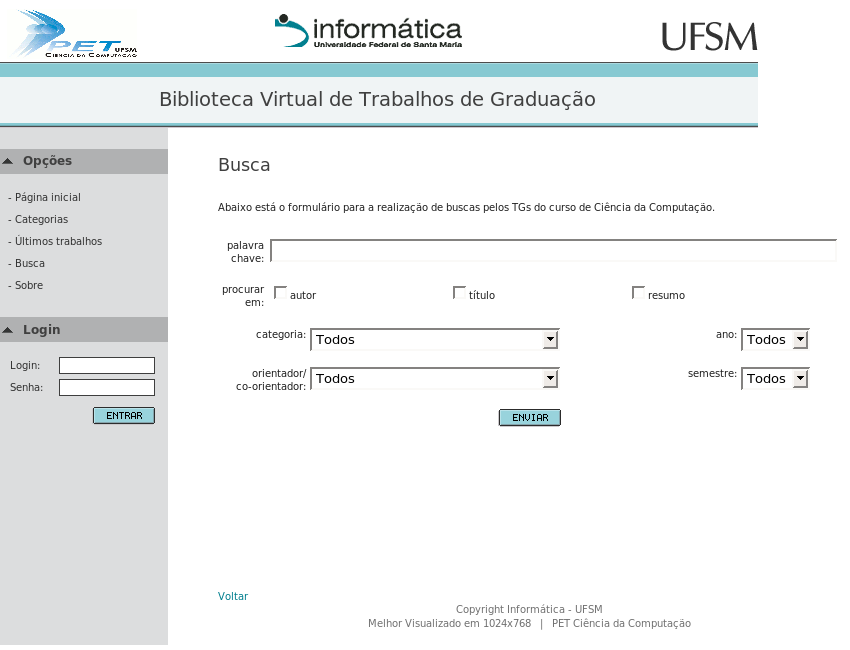
\includegraphics [width = 12cm, height = 12cm]
{img/busca.png}
\caption{P\'{a}gina de Pesquisa de TG's}
\label{f:pesquisa}
\end{figure}

O m\'{o}dulo de administra\c{c}\~{a}o permite dar manuten\c{c}\~{a}o a todos os dados do sistema, como mostra a figura \ref{f:edicao}, na qual o usu\'{a}rio realiza uma altera\c{c}\~{a}o em um TG espec\'{i}fico.

\begin{figure}[ht]
\centering
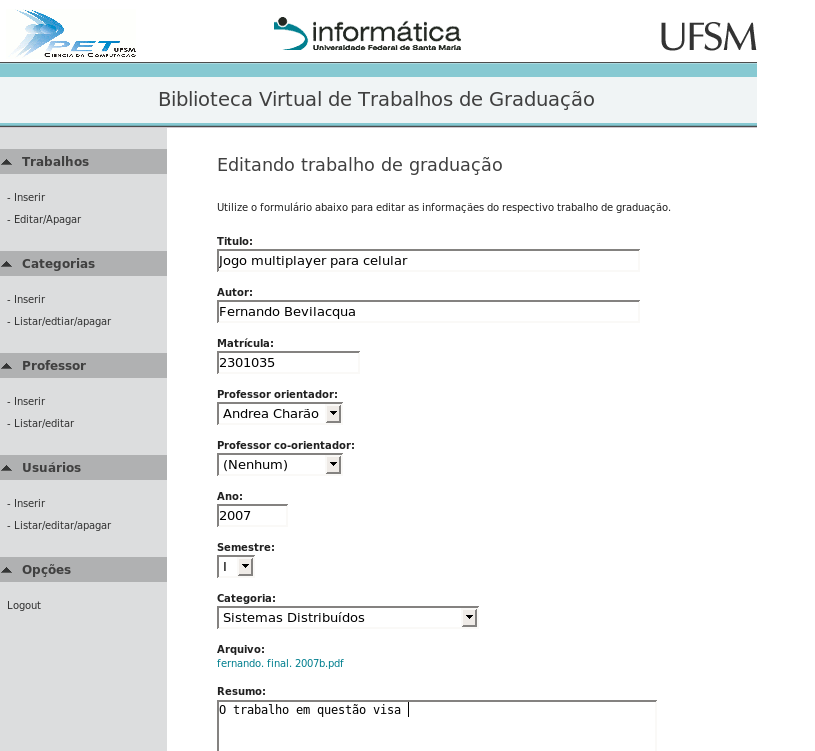
\includegraphics [width = 10cm, height = 8cm]
{img/edicao.png}
\caption{Edi\c{c}\~{a}o dos dados de um TG}
\label{f:edicao}
\end{figure}

O objetivo de fornecer um meio de disponibiliza\c{c}\~{a}o de TG's aos alunos e \`{a} comunidade acad\^{e}mica foi alcan\c{c}ado com sucesso. Atrav\'{e}s do sistema, qualquer pessoa pode ter acesso aos trabalhos de gradua\c{c}\~{a}o disponibilizados pelo curso atrav\'{e}s da Internet. O sistema administrador facilita a manuten\c{c}\~{a}o das informa\c{c}\~{o}es, possibilitando dessa forma que o sistema esteja sempre atualizado.

Outro resultado alcan\c{c}ado foi a cria\c{c}\~{a}o de um sistema  reutiliz\'{a}vel. Os cuidados tomados na fase de planejamento e codifica\c{c}\~{a}o para a cria\c{c}\~{a}o de um sistema gen\'{e}rico, organizado e facilmente alter\'{a}vel permitem que a BDTG seja adaptada a outras situa\c{c}\~{o}es ou casos semelhantes. A BDTG pode ser reutilizada sem grandes altera\c{c}\~{o}es em outros cursos da UFSM ou de outras universidades, apenas modificando-se os arquivos de layout. O sistema tamb\'{e}m pode ser modificado e adaptado a problemas semelhantes, nesse caso, criando alguma classe ou p\'{a}gina de interface do sistema.


\section{Conclus\~{a}o e Trabalhos Futuros}
Este artigo apresentou as etapas do desenvolvimento do BDTG, um sistema para disponibilizar os trabalhos de gradua\c{c}\~{a}o do curso de Ci\^{e}ncia da Computa\c{c}\~{a}o da UFSM. O desenvolvimento desse sistema resultou em duas contribui\c{c}\~{o}es principais: a primeira \'{e} um meio para disponibilizar ao p\'{u}blico em geral os trabalhos desenvolvidos e as atividades realizadas no curso; outra contribui\c{c}\~{a}o \'{e} um sistema cujo c\'{o}digo \'{e} facilmente reutiliz\'{a}vel para situa\c{c}\~{o}es semelhantes ao problema resolvido e a utiliza\c{c}\~{a}o do mesmo por outros cursos e universidades somente alterando os arquivos de configura\c{c}\~{a}o.

Ap\'{o}s a conclus\~{a}o das baterias de testes e a realiza\c{c}\~{a}o das modifica\c{c}\~{o}es e corre\c{c}\~{o}es necess\'{a}rias, o sistema ser\'{a} disponibilizado sob a licen\c{c}a~\nocite{fsf} GNU~\cite{gnu} para que o mesmo seja melhorado e aproveitado por pessoas e organiza\c{c}\~{o}es que t\^{e}m interesse em utiliz\'{a}-lo e adapt\'{a}-lo \`{a}s necessidades espec\'{i}ficas de cada institui\c{c}\~{a}o.

Com trabalhos futuros, pode-se mencionar a expans\~{a}o da BDTG para o armazenamento de Trabalhos de P\'{o}s Gradua\c{c}\~{a}o. Tamb\'{e}m \'{e} poss\'{i}vel a integra\c{c}\~{a}o da biblioteca com a BDTD disponibilizada pelo governo, contribuindo ainda mais para o objetivo do desenvolvimento da mesma. Por fim, pode-se aprimorar as classes bases do sistema a fim de facilitar a personaliza\c{c}\~{a}o das mesmas, disponibilizando-as para outros cursos.

\bibliographystyle{ref/sbc}
\bibliography{ref/bib_tg_sipm_ref}

\end{document}

%% <!-- Local IspellDict: brasileiro -->
%% <!-- Local Variables: -->
%% <!-- mode:flyspell -->
%% <!-- End: -->